\section{Async-flow Interface}
\label{sec:netstar-framework}

%This section gives a detailed introduction to the async-flow interface. The async-flow interface is divided into a manager, which distributes flow packets to different async-flows; and async-flow objects, which can be used for implementing NF logic that need complex asynchronous interactions.

Our major challenge when designing the async-flow interface is how to exploit the power of the future/promise abstraction while exposing easy-to-use interfaces for building NFs. We carefully design a simulated packet processing loop and use returned future objects to concatenate asynchronous operations, to address the challenge.

\subsection{Async-flow Manager}
\label{sec:async-flow-manager}

%The manager is responsible for distributing flow packets to different async-flow objects, creates new async-flow objects when new network flows arrive, and notifies the NF core processing logic the new async-flow objects. %It serves as an entry-point for various L2-L4 NF applications according to \lstinline[style=InlineStyle]{run_async_flow_manager} function defined in Fig.~\ref{fig:netstar-code-sample}.

After a packet is delivered to the async-flow manager from the hook point, the manager first retrieves flow information from the packet header to build a flow key. By default, the flow key is based on the flow 5 tuple (source/destination IP addresses, source/destination port and protocol type) of each TCP/UDP
packet. The manager uses the key to identify an async-flow object from a hash map: if a corresponding async-flow object is found, the received packet is sent to the async-flow object; otherwise, the packet belongs to a new flow, and the manager creates a new async-flow object for the key, and updates the hash map. %, and forwards the packet to the new object.
The manager also configures the new async-flow object % the manager directly reports it to the NF. The NF can then configure the new async-flow object
 with interested events (file hash event)
 %\chuan{add examples}
and core processing logic of the NF, using programming interfaces exposed by the async-flow object.



%Its basic usage has been demonstrated in the \lstinline[style=InlineStyle]{run_async_flow_manager} function in Fig.~\ref{fig:netstar-code-sample}.  has an expressive user interface as shown in Fig.~\ref{fig:netstar-code-sample}. The NF application defines what kind of NF should be created to handle the new async-flow object inside the continuation function, which is called when new flows arrive and new async-flows are created.


%Using the async-flow manager, the NF can acquire newly created async-flow object, register interested events exposed by this async-flow object and run the underlying NF processing logic for the underlying network flow.For a new flow, the manager further encompasses the new async-flow object and the new flow packet inside a context object, which is referred to as a new {\em flow context}. The new flow context is placed into a queue. The NF core processing logic is then notified to fetch the new flow context from the queue.

%For each new async-flow object, the manager first configures what events should be reported to the core NF processing logic from the preprocessor. Then the manager registers a packet handler function that implements the core NF processing logic to the async-flow object.


% configures the core NF processing logic by registering a packet handler function to the async-flow object. %implemented inside a registered packet handler function.
%and the core NF processing logic with xxx

%\chuan{I cannot understand how the notification is done based on the following descriptions and the future/promise introduction in Sec. 2. Revise carefully by specifying what is exactly the future object (value of the type) and continuation function (capture variables), what the continuation function does, and if any promise object is associated with the future object. Don't point to the example in Fig.~\ref{fig:netstar-code-sample}, but describe in general} The notification process is done via a special future object, which becomes available when the queue is not empty. This future object is returned to the NF application with \lstinline[style=InlineStyle]{on_new_async_flow} as shown in Fig.~\ref{fig:netstar-code-sample}. The NF application can append a continuation function to this future object like line 3 in Fig.~\ref{fig:netstar-code-sample}. This continuation function is only invoked when the queue that holds the new flow context is not empty, therefore the NF application can retrieve a new flow context within this continuation function and initiates the NF processing logic for this flow shown in line 4 to 9 in Fig.~\ref{fig:netstar-code-sample}. Eventually, when the new flow object obtained in the continuation function is destroyed, the first flow packet is delivered to the async-flow object.

%by calling \lstinline[style=InlineStyle]{cur_async_flow} as in Fig.~\ref{fig:netstar-code-sample}, construct an application-level object like \lstinline[style=InlineStyle]{malware_detector} as in Fig.~\ref{fig:netstar-code-sample}, register interested events for this application-level object to handle and eventually initiates the entire NF processing logic by registering a new loop function as shown in line 8 and 15 in Fig.~\ref{fig:netstar-code-sample}.

\subsection {Async-flow Object}
\label{sec:async-flow-object}

\begin{figure}[!h]
\centering
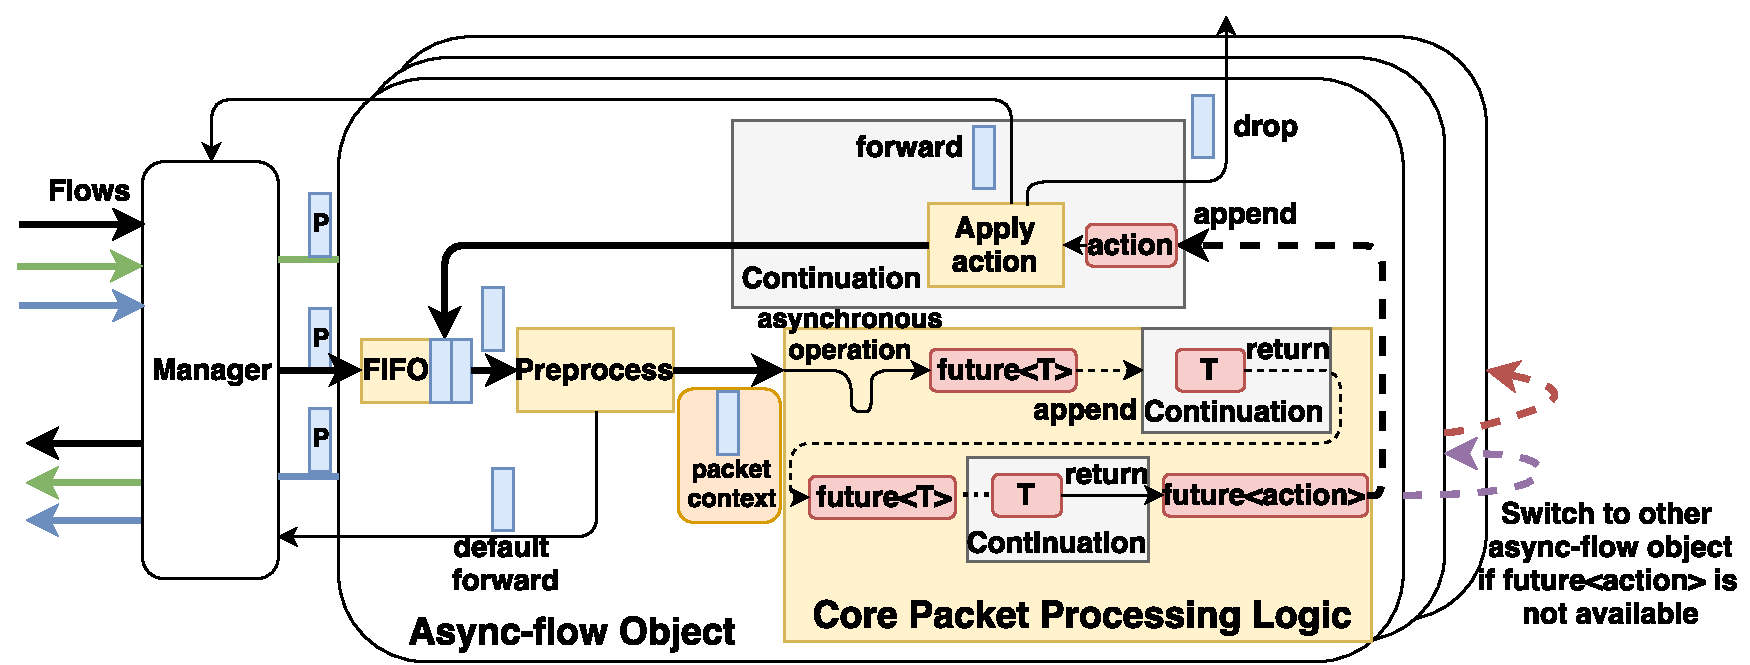
\includegraphics[width=\columnwidth]{chap-netstar/figure/async-flow-object.pdf}
\caption{Workflow of async-flow objects (P represents a packet).}
\label{fig:simulated_loop}
\end{figure}

The async-flow objects are key components to implement asynchronous packet processing in an NF. We target the following design objectives in its design.
(1) \textbf{Ease of Use.} The exposed programming interfaces should be easy to use, especially for programmers to implement NFs.
(2) \textbf{Full Processing Asynchrony.} %Asynchronous packet/flow processing should be fully supported.
After an async-flow object launches an asynchronous operation when processing a packet, it should yield its execution immediately to other async-flow objects, without blocking.

% To handle flow asynchronous, the async-flow object or the \netstar~framework should ...; to handle request asynchrony, ...
% In particular, when the NF application performs an asynchronous operation, the async-flow object should properly preserve the current processing context and the NetStar framework should switch to process other meaningful tasks. On the other hand, the exposed interface should be well integrated with future/promise abstraction to simplify asynchronous programming.

%For each new async-flow object, the manager first configures what events should be reported to the core NF processing logic from the preprocessor. Then the manager registers a packet handler function that implements the core NF processing logic to the async-flow object.

In \netstar, the programming interfaces exposed by the async-flow object to a programmer include an interface for registering a special packet handler function that implements the core NF processing logic, and an interface for configuring what events to be reported to the registered packet handler function. % from the preprocessor.
 The interfaces are easy to use: registration of a packet handler function %the function is regularly invoked by the async-flow object to process the received packet,
 is very much the same as implementing a packet handler in existing NF architectures~\cite{bro, snort}.

%xxx  We achieve design objective 1 above by ... exposing xxx that the NF programmer can register xxx with, such that the event ... and the core processing logic can be regularly invoked to process the received packet, in the same way of implementing a packet handler as in many existing NF architectures \cite{}.
%We can make async-flow object expose a loop function for the NF application to register. The loop function can then be regularly invoked to process the received packet, like a regular packet handler seen in many existing NF architectures \cite{}.

To achieve the second objective, we strategically simulate a packet processing loop within each async-flow object via a series of future-continuation chains, pause a packet processing loop if any intermediate future object is unavailable, and only resume it when the future object becomes available. %The simulated packet processing loop keeps running by recursively invoking the entry point of the simulated loop from a continuation function.
An illustration of the workflow within and among async-flow objects is presented in Fig.~\ref{fig:simulated_loop}.

%If the loop function is directly implemented as a regular packet handler function, then the loop function can only execute asynchronous operations via extensive use of callback functions, which complicates asynchronous programming.
% loop function returning a future object containing an action decision, and simulate a packet processing using the returned future object.

%\subsubsection{Simulated Packet Processing Loop} We discuss how the simulated packet processing loop work by tracing the execution of a flow packet as shown in Fig.~\ref{fig:simulated_loop}.
%In each async-flow object, we simulate a packet processing loop. %\chuan{explain why you say `simulate' or `simulated' packet loop, what are you simulating?}.
%After the packet is delivered to the async-flow object from the manager, the async-flow object checks whether the simulated packet processing loop is running. If so,

\vspace{1mm}
\noindent\textbf{FIFO Queue.} When a packet is sent from the manager to the async-flow object, the packet is first pushed into an FIFO queue and waits to be fetched by the packet processing loop. %Otherwise, async-flow object launches the simulated loop to process the packet.

\vspace{1mm}
\noindent\textbf{Preprocessing.} When a packet goes into the packet processing loop,  it is first preprocessed to generate a set of events. %This design is inspired by mOS \cite{}, as the arrival of a packet may trigger more interested events after preprocessing than the packet arrival itself.
 For instance, if an in-sequence TCP packet arrives, the preprocessing may retrieve new payload from the reordering buffer to reconstruct the TCP byte stream and report it as an new event, along with arrival event of the TCP packet. In this way, some functionalities within the core processing logic can be offloaded to the preprocessing step for simplification. \netstar~is equipped with four default preprocessors: a simple UDP preprocessor and a simple TCP preprocessor report packet arrival events; a TCP tracking preprocessor reports events on TCP packet arrival, TCP connection status change and the reconstruction of the TCP bytestream; a file extraction preprocessor extracts transmitted files from the byte stream and reports hash values of the files as events. All four preprocessors are equipped with a timer to report flow time-out events, when the async-flow object can gracefully shut down its packet processing loop.


After preprocessing, a packet {\em context} object is constructed, containing the current packet and all the generated events. If none of the events matches any of the events that the NF is interested in (\eg, an IDS may only be interested in reconstructed TCP byte stream, not the arrival of an out-of-order TCP packet), a default action is performed, \ie, forwarding the packet out (to the next-hop NF or the flow destination), and another packet is fetched for preprocessing from the FIFO queue; otherwise, the packet context is sent to the core processing logic for further processing.

%\subsubsection {Preprocessing and event extraction.}
%\label{sec:preprocessing-event-extract}


%\textcolor{blue}{The purpose of the preprocessing layer is to extract interested events, %(chuan: no need to mention) as inspired by mOS \cite{},
%including flow timeout events, packet arrival events, and other possible events that the NF application would like to tackle. Currently, the preprocessing later is implemented as a C++ template. NetStar provides three default preprocessors. A simple UDP preprocessor and a simple TCP preprocessor are used to report only packet arrival event and flow timeout event. A TCP tracking preprocessor is used to report events about TCP connection status change and reconstruction of the TCP bytestream.}


%\textit{First,} returning a future object from the loop function enables programmers to utilize future/promise abstraction. To concatenate an asynchronous operation, the programmer can initiate a asynchronous operation first, and then within the continuation function, returns the future object containing the action decision. According to the properties define in Sec.~\ref{}, the resulting future object still contains an action decision, but it will only become available when the asynchronous operation ends.




\vspace{1mm}
\noindent\textbf{Core Packet Processing Logic.}
In the core processing logic, events from the packet context are retrieved and packet processing logic is executed together with a number of asynchronous operations, carried out through a chain of future/promise objects and continuation functions. To handle one asynchronous operation, a future object is constructed, associated with a promise object, and a continuation function is appended to the future object. When the promise object turns the future object into available state (when the asynchronous operation is completed), the appended continuation function is invoked, which carries out corresponding processing based on the received response and returns another future object for handling the next asynchronous operation. Multiple asynchronous operations can be handled using such a `future/promise-continuation' chain.

%For instance, a firewall may check for the event of new packet arrival, retrieve the header of the packet and compare it against an access-control-list.

Using malware detection in IDS as an example, the core processing logic includes two asynchronous operations: querying the local database and querying the MHR. A future object is first constructed to receive query response from the local database, and the database response is obtained as the concrete type of value in the future object. A promise is associated to turn the future into available state when the response returns. The appended continuation function is invoked then, and returns another future object, which receives query response form the MHR. The second future object obtains the MHR response as its concrete type of value and passes it to an appended continuation function, which may raise an alert in case that the response indicates the detection of a malware.


\vspace{1mm}
\noindent\textbf{Final Future Object and Its Continuation Function.} The last continuation function in the asynchronous `future/promise-continuation' chain is forced to return a future object containing an action decision (\eg, drop or forward in the malware detection example). This future object becomes available when all asynchronous operations in the core processing logic have been completed. A continuation function is appended to this future object, which receives the action decision from the future object and carries out the action accordingly (\eg, drops the packet or forwards it to the next hop. The current packet context is then destroyed, and the packet processing loop moves on to fetch another packet from the FIFO queue (if it is not empty), and recursively restarts itself.

%\vpsace{1mm}
\vspace{1mm}
\noindent\textbf{Timeout of Async-flow Object and Safety Guarantee.} When the flow handled by the async-flow object eventually becomes idle, a timeout event is triggered, which stops the packet processing loop and transforms a future object into ready state. This future object is used to receive the timeout notification and the continuation function appended to it does the actual clean up task, which deallocates the async-flow object and other auxiliary objects used by the async-flow object. This mechanism guarantees that whenever the packet processing loop runs, the async-flow object and other auxiliary objects used by it are always safe to visit.


\vspace{1mm}
\noindent\textbf{Switching to Another Async-flow Object.} After an async-flow object has issued an asynchronous operation, the thread that the async-flow interface is running in moves on to handle another async-flow object, \ie, the packet processing loop in another async-flow object starts to fetch packets from its own FIFO queue and processes them. Different async-flow objects implement exactly the same logic in an NF. The programming style in implementing packet processing logic is very much like synchronous programming, while full asynchronous packet processing can be achieved. %All these attribute to our effective interface design based on the future/promise paradigm.
% we effectively utilize future object transformation provided by future/promise abstraction (see Sec.~\ref{sec:tranform-future-object}).


%\textbf{Return \lstinline[style=InlineStyle]{future<action>}.} By returning \lstinline[style=InlineStyle]{future<action>}, whether to forward or drop the packet is offloaded to the async-flow object. The async-flow object can append another continuation to the returned \lstinline[style=InlineStyle]{future<action>}: when \lstinline[style=InlineStyle]{future<action>} becomes available, then the loop function has finished all asynchronous processing and the async-flow is safe to forward or drop the packet depending the action decision contained in \lstinline[style=InlineStyle]{future<action>} and destroy the current packet context.

%\textbf{Run Simulated Loop Again.} During the execution of this simulated loop, new packets may arrive and get enqueued into the FIFO. To handle these packets, the simulated loop needs to be started again. This is also done in the continuation function appended to \lstinline[style=InlineStyle]{future<action>}: after applying packet forwarding decisions, if the FIFO is not empty, the async-flow object calls the entry function of the simulated loop again to restart the simulated loop.



%The second goal
%If the loop function is implemented as a regular packet handler, the loop function can only achieve this goal via extensive use of callback functions, which violates the principle of ease of use. Our solution is to let the loop function returns a future object containing an action decision about what to do with the currently processed packet. This solution is neat in several aspect:

%\textit{First,} returning a future object from the loop function enables programmers to utilize future/promise abstraction. To concatenate an asynchronous operation, the programmer can initiate a asynchronous operation first, and then within the continuation function, returns the future object containing the action decision. According to the properties define in Sec.~\ref{}, the resulting future object still contains an action decision, but it will only become available when the asynchronous operation ends.

%\textit{Second,} by returning an action decision, we offload the decision to forward or drop packet to the async-flow object. Therefore we can easily save all related context information, including the current packet and the exposed packet, within the async-flow object. To track this context information, we can simply saves a pointer to the container object like the malware\_detector object shown in Fig.~\ref{}.

%\textit{Third,} this allows us to simulate a packet processing loop. The async-flow object can append another continuation function to the future object returned from the loop function. Inside this continuation function, the async-flow object can recursively call loop function again to simulate a real loop function.


%A regular packet handler can only achieve this goal via extensive use of callback functions, which may

%For a regular packet handler function, it is hard to accomplish th

% Async-flow object exposes an iterative function which can be used by NF application to implement the core NF processing logic. The async-flow object also delivers various events, including flow time out and packet arrival event to the NF application. Most importantly, the design of the iterative function preserves the power of future/promise abstraction: the NF application can carry out arbitrary asynchronous operations inside the async-flow object with ease as illustrated in Fig.~\ref{fig:code-sample}.

%\subsubsection {Exposed Interface.} The async-flow object exposes two kinds interfaces for the NF applications.

%\textbf{An Iterative Function.} When a new async-flow object is created, NF application should register an iterative function to the async-flow object, which is called when interested new events happen. Inside the iterative function, the NF application can use the async-flow to query the current interested events and implement NF processing logic. The only restriction that NetStar impose on the iterative function is the type of its return value (via C++ compiler type checking). The iterative function must return a future objection containing an action result. When the future becomes ready, the async-flow knows how to perform post-processing about the current events.

%\textbf{Event Query.} The async-flow is equipped with a customizable preprocessing layer, which performs preprocessing to the received packet and generate an event for the iterative function to handle. The iterative function uses the event query interface exposed by async-flow to query and handle the event. This is inspired from the event system design of mOS \cite{}.

%\subsubsection {Simulated loop.} The async-flow achieves its functionality by running a simulated loop. By loop, we mean that the iterative function provided by the user will be sequentially invoked for each received flow packet. By simulated, we mean that we are not actually running a regular \lstinline[style=InlineStyle]{for} loop or \lstinline[style=InlineStyle]{while} loop in C++. If the async-flow runs a real loop, NetStar loses all the possible flow-level asynchrony, as multiple loops can not be scheduled within a single thread without using coroutine (see Sec.~\ref{}). In that case, only a single loop can run and consume all the thread execution time.

%The simulated loop is implemented by recursively calling the \lstinline[style=InlineStyle]{simulated_loop} function from a continuation function as shown in line 21 in Fig.~\ref{fig:simulated_loop}.

%Initially, the simulated loop is not launched and the async-flow waits for new packets. Once new packet is received, async-flow calls \lstinline[style=InlineStyle]{on_new_packet} function to launch the simulated loop (line 1). Since each async-flow object can only own a single simulated loop, we use a fifo queue to buffer the packet if the simulated loop is running and processing other flow packets (line 2). The simulated loop is restarted again if it not running when async-flow receives a new packet (line 5-6).

%After the packet is preprocessed and the event context is constructed (line 11-14), the iterative function is called for processing the event. Remember that the iterative function returns a future object containing an action result. We immediately chain a continuation function to this future object, which calls recursively calls the \lstinline[style=InlineStyle]{simulated_loop} function.

%Before the future object returned by the iterative function becomes ready, all the newly received packets will be pushed back into the fifo queue. Therefore the iterative function is free to carry out any kind of asynchronous operations. When the iterative function blocks and waits for an event to happen, the NetStar framework simply switches to other meaningful. Eventually, when the future object becomes available, \lstinline[style=InlineStyle]{simulated_loop} is called again to process other packets received when the async-flow is blocked.

%In Seastar, the continuation function is an heap-allocated function object and pushed to an execution queue for invocation, therefore recursively call a function within the continuation function will not cause errors like stack overflow.
